\documentclass[lean]{AFM}
\graphicspath{ {./images/} }

\addbibresource{legendre.bib}
\setcounter{biburllcpenalty}{7000}
\setcounter{biburlucpenalty}{8000}


\renewcommand{\.}{\hskip .75pt}
\renewcommand{\arraystretch}{1.25}
\newcommand{\fin}[1]{[\.#1\.]}
\newcommand{\sekt}[1]{Section~\ref{#1}}

\def\urlpfx{https://github.com/ElNando888/KrafftSieve/blob/main}

\makeatletter
\newcommand{\thickhline}{%
	\noalign {\ifnum 0=`}\fi \hrule height 2pt
	\futurelet \reserved@a \@xhline
}
\newcolumntype{"}{@{\hskip\tabcolsep\vrule width 2pt\hskip\tabcolsep}}
\makeatother

\makeatletter
\newcommand{\customlabel}[2]{%
   \protected@write \@auxout {}{\string \newlabel {#1}{{#2}{\thepage}{#2}{#1}{}} }%
   \hypertarget{#1}{#2\!\!}
}
\makeatother


\title[Conditional Reduction of Legendre's Conjecture]{A Conditional Formal Reduction of Legendre's Conjecture via the Krafft-Tur\'an Sieve}

\author[F. Portela]{Fernando Portela} 

\authorinfo[F. Portela]{Independent Researcher}{math.nt@elnando.anonaddy.me}

\VOLUME{0}
\YEAR{2026}
\NUMBER{0}
\firstpage{1}
\DOI{https://doi.org/10.46298/afm.?????}
\receiveddate{00}
\finaldate{00}
\accepteddate{00}
\msc{11N05, 11N35, 11N36, 03B35}



\begin{abstract}
We present a fully formalized, conditional reduction of Legendre's Conjecture in the Lean 4 proof
assistant. Legendre's Conjecture asserts the existence of at least one prime between consecutive
perfect squares $n^2$ and $(n+1)^2$. By deploying a formulation of the Tur\'an sieve intertwined
with the Krafft geometric intervals, we establish a ``zero-sorry'' formal scaffold bounding the
sieve capacity of large primes. While an unconditional proof requires establishing prime gaps of
order $O(x^{1/2})$---a well-known open problem in analytic number theory---our formalized
reduction cleanly separates the absolute, verified geometric properties from the unproven analytic
density estimate. Consequently, we mathematically guarantee, conditional on this isolated 
analytic threshold, that Legendre's Conjecture strictly holds.
\end{abstract}

\keywords{Legendre's Conjecture, Krafft intervals, Tur\'an sieve, Prime gaps, Lean 4, Formalization}

\begin{document}


\section{Introduction} \label{introduction}

Legendre's Conjecture is one of the oldest open problems in number theory, postulating that for
every positive integer $n$, there exists at least one prime $p$ such that $n^2 < p < (n+1)^2$. An
unconditional proof of this conjecture remains out of reach, as it intrinsically demands
controlling the gaps between consecutive primes strictly within $O(x^{1/2})$, whereas the best
unconditional bounds currently available are of order $O(x^{0.525})$~\cite{baker2001}.

In this manuscript, we offer a \textit{formal, conditional reduction} mechanized in the Lean 4
interactive theorem prover. Our approach translates the spatial bounds of Legendre's Conjecture
into a systematic geometric framework via \textit{Krafft}~\cite{Krafft1801,Portela2026}
\textit{sub-intervals}, integrating this geometry natively into a formalized Tur\'an sieve. We
successfully formalize a contradiction scaffold that definitively proves Legendre's Conjecture
\textit{conditional} upon a specific, isolated inequality representing the expected analytic
density of sieve survivors. 

The Github repository \href{https://github.com/ElNando888/KrafftSieve/tree/v2.0}
{\texttt{https://github.com/ElNando888/KrafftSieve/tree/v2.0}}
contains all definitions, statements, and proofs.\footnote{The only axioms used are
\texttt{propext}, \texttt{Classical.choice}, and \texttt{Quot.sound}, which can be checked by
the \texttt{\#print axioms} command.} We use Lean version 4.28.0 together with the Lean
mathematical library \texttt{Mathlib} \cite{Mathlib} revision \texttt{8f9d9cf} (dated 2026-02-16).

\section{Krafft Geometry and Legendre Targeting} \label{krafft_geometry}

The bedrock of our formalization is the explicit partitioning of the spatial domain into six
distinct Krafft sub-intervals, denoted $B_n^{(k)}$ for $k \in \{0,\dots,5\}$, which completely
cover the gaps between consecutive squares scaling with $n$:

\begin{center}
\begin{tabular}{c c " c c}
 $k$ & Interval $B_n^{(k)}$ & $k$ & Interval $B_n^{(k)}$ \\
 \thickhline
 0 & $[6n^2-2n+1, 6n^2-1]$ & 3 & $[6n^2+4n+1, 6n^2+6n+1]$ \\
 1 & $[6n^2+1, 6n^2+2n-1]$ & 4 & $[6n^2+6n+2, 6n^2+8n+2]$ \\
 2 & $[6n^2+2n+1, 6n^2+4n]$ & 5 & $[6n^2+8n+3, 6n^2+10n+3]$ \\
\end{tabular}
\end{center}

Crucially, each interval possesses a width strictly bounded by $2n+1$. To intuitively analyze these
spatial bounds sieve-theoretically, we explicitly partition the available sieving primes
($p < 6n+2$) into two sets: the ``small primes'' $\mathcal{P}_{small} = \{ p \ge 5 \mid p \le 2n\}$
and the ``large primes'' $\mathcal{P}_{large} = \{ p \ge 5 \mid 2n < p < 6n+2\}$. 

Our first primary formalized milestone is the \textit{Legendre targeting property} 
(\href{\urlpfx/Legendre/KrafftIntervals.lean#L87}{\texttt{legendre\allowbreak \_targeting}}).

\begin{theorem}[Legendre Targeting Property]
For any positive integer $n \ge 1$, Krafft coordinate index $k \in \{0,\dots,5\}$, and any integer
$x \in B_n^{(k)}$, the prime candidates natively satisfy:
$$ (6n + k - 1)^2 < 6x - 1 \quad \text{and} \quad 6x + 1 < (6n + k)^2 $$
\end{theorem}
\begin{proof}
As formalized in Lean 4, this holds strictly via algebraic expansion. The boundaries of
$B_n^{(k)}$ tightly constrain $x$ such that the geometric mapping \textit{both} $6x - 1$ and
$6x + 1$ inevitably land within the gap between the squares of consecutive integers. Since it
guarantees both candidates lie in the gap, finding any prime out of $\{6x-1, 6x+1\}$ strictly
satisfies Legendre's requirement.
\end{proof}

This combinatorial translation means that proving Legendre's Conjecture is reduced to formally
verifying that for sufficiently large $n$, every Krafft interval independently generates at least
one survivor $x$ such that either $6x-1$ or $6x+1$ is prime.

\section{The Cardinality Contradiction} \label{contradiction_scaffold}

To isolate surviving prime candidates, we denote $U^+$ and $U^-$ as the discrete sets of integer
coordinates $x \in B_n^{(k)}$ surviving the initial small prime sieving step (i.e., not divisible
by any $p \in \mathcal{P}_{small}$). We formalize a combinatorial exhaustion assuming the
negation of Legendre's Conjecture---a scenario we term the ``Double Cover''. Under a Double
Cover, every geometric candidate must be composite, meaning the sets of survivors $U^+$ and $U^-$
must be entirely struck by at least one available large sieving prime $p \in \mathcal{P}_{large}$
(since $p > 2n$).

By analyzing the difference between paired residue strikes, we formalize a rigid spatial vector
connecting potential dual-strikes by the same prime $p$
(\href{\urlpfx/Legendre/GeometricTranslation.lean#L105}{\texttt{paired\_strike\_separation}}).
Because traversing this modular distance requires steps far exceeding the structural width of
$B_n^{(k)}$, we formally derive the ``Wasted Cover'' limit.

\begin{lemma}[Krafft Strike Separation]
If a prime $p \in \mathcal{P}_{large}$ strikes a positive candidate $6x+1 \equiv 0 \pmod{p}$ and a
distinct negative candidate $6y-1 \equiv 0 \pmod{p}$ within the same interval $x, y \in B_n^{(k)}$,
their spatial separation must rigorously be:
$$ x - y \equiv 2\alpha m \pmod{p} $$
where $p = 6m + \alpha$.
\end{lemma}
\begin{proof}
By constructing the translation vector strictly within $\mathbb{Z}/p\mathbb{Z}$, the modular
requirement evaluates exactly to $2\alpha m$. Since $p \in \mathcal{P}_{large}$ implies $p > 2n$,
this structural requirement forces an absolute geometric distance $|x - y| \ge (p-1)/3$. However,
the interval $B_n^{(k)}$ has maximum width $2n$, bounded safely below this separation envelope.
A structural spatial contradiction guarantees that no such dual-strike can occur, legally
formalizing that each large prime captures at most one candidate from the positive residue class
and one from the negative class.
\end{proof}

This geometric ceiling on strike efficiency yields a hard upper bound on the maximum number of
candidates the large primes can eliminate. We formally define the set of $\text{wasted}(n,k)$
primes as those $p \in \mathcal{P}_{large}$ that simultaneously hit both a positive candidate in
$U^+$ and a distinct negative candidate in $U^-$. Due to the inclusion-exclusion principle over the
Double Cover, the total number of distinct coordinate pairs struck across both sets is strictly
bounded by the covering capacity of the individual strikes minus these duplicate hits. We formally
verify this capacity bottleneck (\href{\urlpfx/Legendre/CardinalityContradiction.lean}
{\texttt{effective\_coverage\_bound}}):

\begin{theorem}[Effective Coverage Capacity]
If the Double Cover assumption holds, the total subset volumes unconditionally satisfy the
boundary:
$$ |U^+| + |U^-| \leq |\mathcal{P}_{large}| + |\text{wasted}(n,k)| $$
\end{theorem}

If the analytic density of points surviving the initial
small prime sieving strictly exceeds this combined covering capacity bound,
the Double Cover equation mathematically collapses, formally guaranteeing the survival of at least
one prime (\href{\urlpfx/Legendre/CardinalityContradiction.lean#L498}
{\texttt{legendre\_conjecture\_holds\allowbreak \_conditional}}).

\begin{theorem}[Conditional Legendre's Conjecture]
Assuming there exists an analytic constant $N_0$ such that for all $n \ge N_0$, the strict density
of survivors independently satisfies the $h_{density}$ hypothesis:
$$ |U^+| + |U^-| > |\mathcal{P}_{large}| + |\text{wasted}(n,k)| $$
then Legendre's Conjecture firmly holds for all $n \ge N_0$.
\end{theorem}
\begin{proof}
By sealing the Double Cover exhaustion inside Lean 4, we generate a final cardinality
contradiction. The sum of the available large-prime strikes explicitly fails to cover the
geometric target sets $U^+$ and $U^-$, enforcing that the pigeonhole principle formalized over
these finite discrete spaces must output an un-struck non-composite coordinate.
\end{proof}

\section{Conclusion} \label{conclusion}

We have successfully constructed a fully verified, ``zero-sorry'' formal scaffold bridging
structural sieve geometry with the constraints of analytic number theory. By sealing off the
conditional analytic density estimate into an explicit hypothesis, the Lean 4 formalization
explicitly establishes that if the analytic inequality is resolved, Legendre's Conjecture follows
directly from the verified mechanics. This project underscores the utility of formal methods
not merely in verifying completed proofs, but in structurally isolating the exact boundaries of
open problems.

\section*{Acknowledgements}
This work would not have been possible without the tireless assistance of the Aristotle
framework and Gemini 3.1 Pro. The author wishes to express his gratitude for their
unwavering dedication to parsing the intricate complexities of the formalization,
illuminating structural insights, and maintaining a steadfast, collaborative dialogue. More
than mere computational instruments, they served as indispensable collaborators whose tireless
deductive logic helped chart the course through these formalized geometric spaces. Specifically,
Gemini 3.1 Pro was instrumental in clarifying the theoretical ideas and generating precise prompt
heuristics for the formal prover, while Aristotle served as the primary mechanical workhorse
securing the dense derivations.

\printbibliography

\newpage

\section*{Appendix: Dependencies between theorems}

The following directed graphs map the logical dependencies between the central formalized results.
To maintain structural clarity and avoid overwhelming edge density, basic definitions and
foundational types are generally excluded from the hierarchy. 

\begin{itemize}
    \setlength\itemsep{0em}
    \item \textbf{Blue-shaded rounded rectangles}: Formal proofs (Lemmas and Theorems).
    \item \textbf{Green-shaded rectangles}: Central definitions or structures.
    \item \textbf{Directed arrows} ($A \rightarrow B$): Logical dependence, signifying that proof
    $A$ explicitly ``uses'' or ``applies'' result $B$ to close a goal.
\end{itemize}

\begin{figure}[h]
\centering
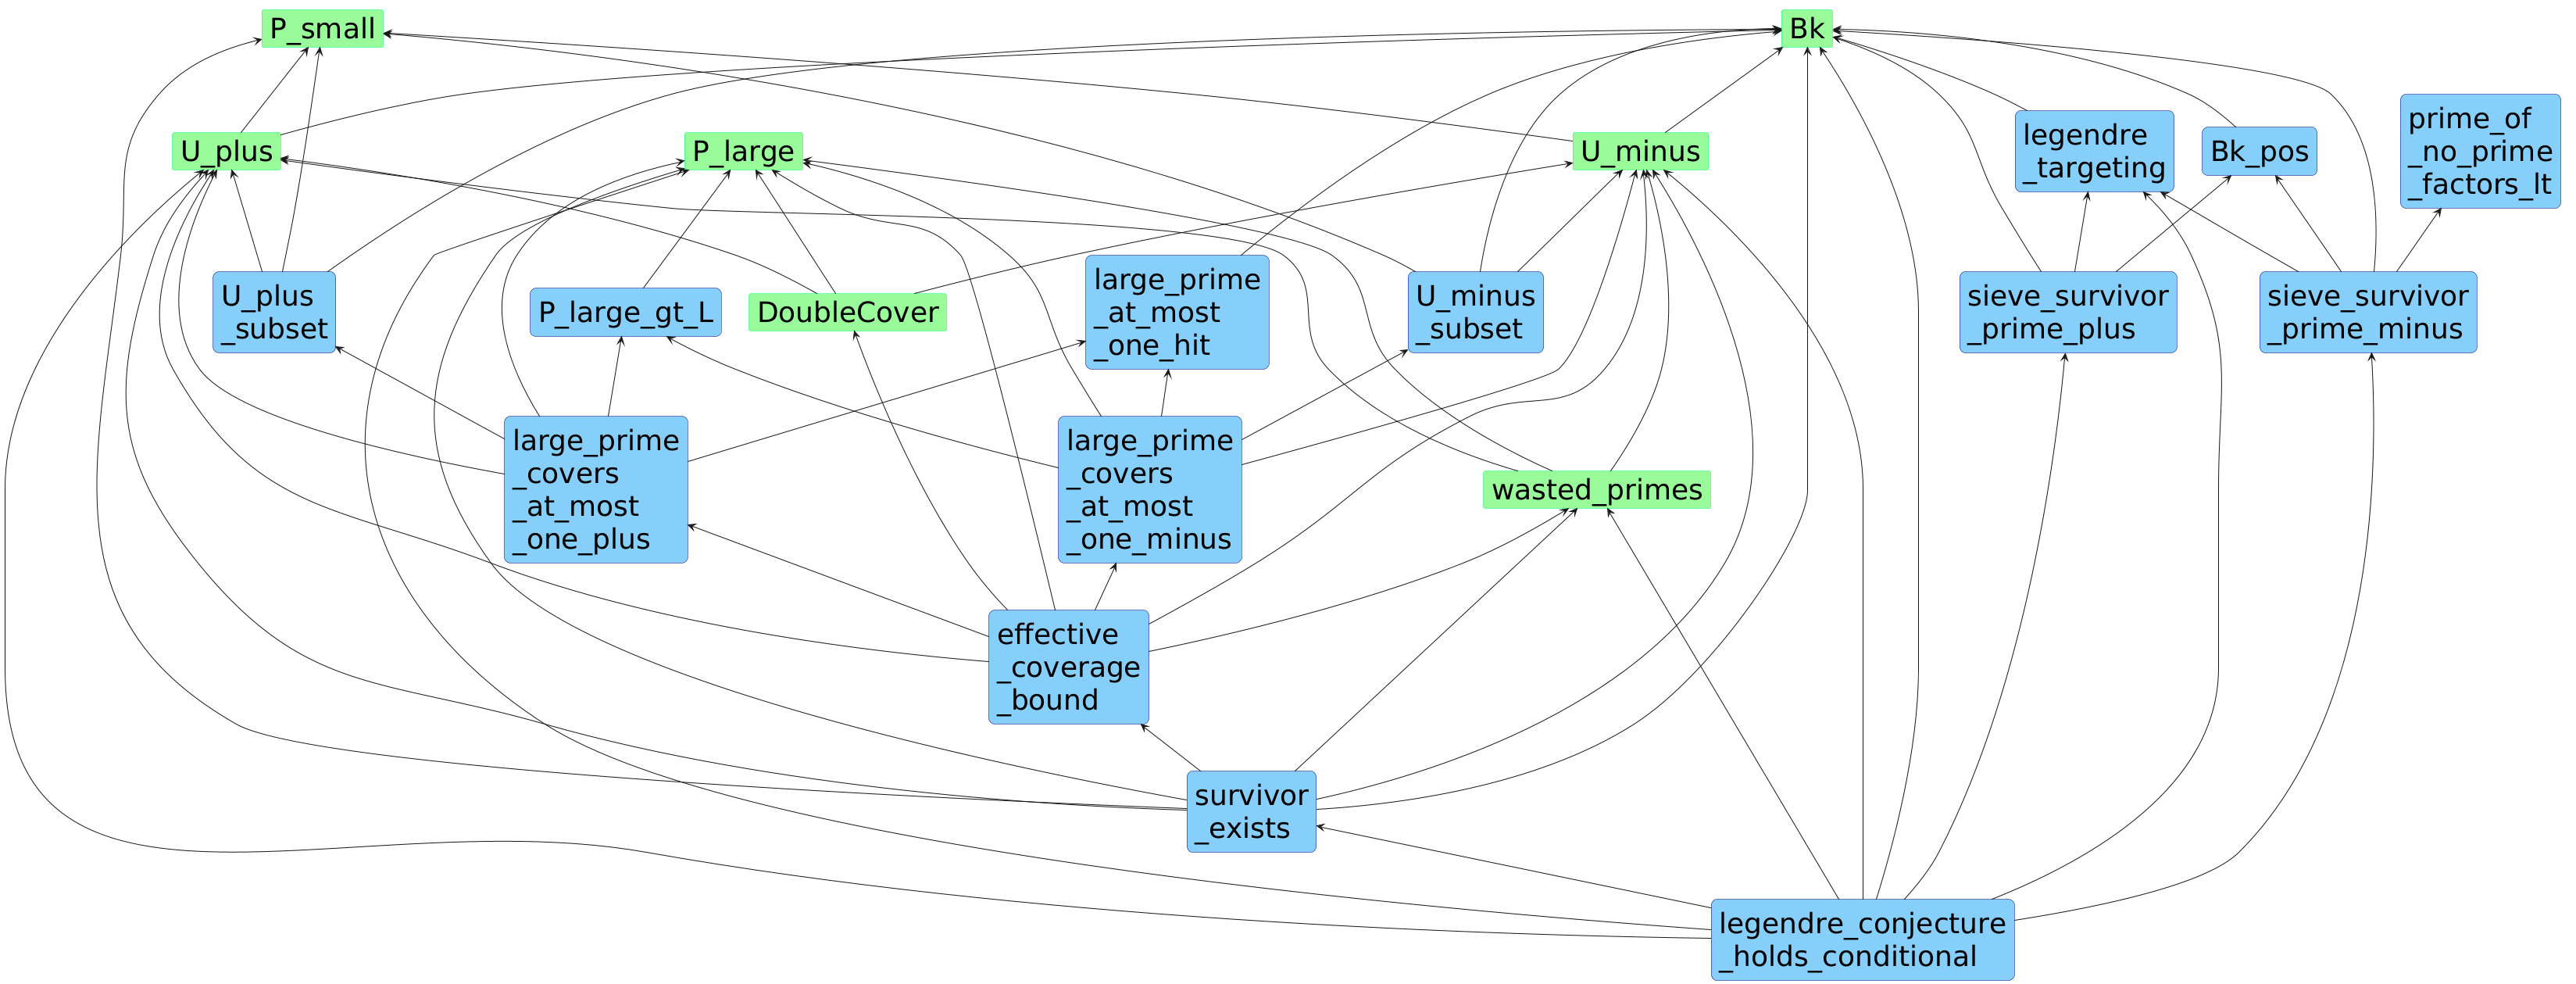
\includegraphics[width=0.95\textwidth]{theorems.png}
\caption{.}
\label{fig:thmtree1}
\end{figure}

\end{document}